\section{平均场逼近}
\label{sec:dapx-mean-field}

高维目标难算，往往是因为各分量纠缠在一起：求一个分量的边缘，要对其余所有分量的联合取值求和。如果候选分布让各分量独立，很多计算就拆成了一维的计算。把变量分成$m$组$\bm{x}=(x_1,\dots,x_m)$，$x_j\in\mathcal{X}_j$（每组可以是一个分量，也可以是几个分量），参考测度取各组参考测度的乘积，候选限制为
\begin{equation}
 q(\bm{x})=\prod_{j=1}^{m}q_j(x_j) ,
 \label{eq:dapx-product}
\end{equation}
其中每个因子$q_j$可以是$\mathcal{X}_j$上任意一个概率密度。用这种乘积分布逼近目标，称为\term{平均场逼近}（mean-field approximation）。名称来自统计物理：每个分量感受到的是其余分量的平均作用，下一小节的更新公式正是如此。

这里的限制只有一条：组与组之间独立。每个因子本身不限于任何参数族，可以是任意形状。所以“乘积”与“有限维参数化”是两回事：前者限制的是依赖结构，后者限制的是每个分布的形状。本节先看独立性限制本身的后果，再推导按候选加权的方向下逐个因子求最优的更新。

先处理比较简单的一个方向。按目标加权时，最优的乘积分布就是目标的边缘乘积，并且最小值正是第~\ref{chap:information-measures}章的互信息。

\begin{lemma}[正向KL下的最优乘积]
\label{lem:dapx-forward-product}
设$m=2$，目标$\Pi$有边缘$\Pi_1,\Pi_2$，且互信息有限：
\begin{equation}
 I(X_1;X_2)=D_{\mathrm{KL}}(\Pi\Vert\Pi_1\otimes\Pi_2)<\infty .
 \label{eq:dapx-mi-finite}
\end{equation}
则对任意因子$Q_1,Q_2$，
\begin{equation}
 D_{\mathrm{KL}}(\Pi\Vert Q_1\otimes Q_2)=I(X_1;X_2)+D_{\mathrm{KL}}(\Pi_1\Vert Q_1)+D_{\mathrm{KL}}(\Pi_2\Vert Q_2) .
 \label{eq:dapx-forward-product}
\end{equation}
因此最优乘积唯一，是$\Pi_1\otimes\Pi_2$，最小值是$I(X_1;X_2)$。
\end{lemma}

\begin{proof}
若$\Pi_1\not\ll Q_1$，则有集合$A$使$\Pi_1(A)>0=Q_1(A)$，于是
\[
 \Pi(A\times\mathcal{X}_2)>0=(Q_1\otimes Q_2)(A\times\mathcal{X}_2) ,
\]
两边都是$+\infty$；$\Pi_2\not\ll Q_2$同理。下设$\Pi_j\ll Q_j$，密度记为$\pi_j,q_j$。由$I<\infty$知$\Pi\ll\Pi_1\otimes\Pi_2$，于是$\Pi\ll Q_1\otimes Q_2$，并且在$\Pi$几乎处处成立
\[
 \ln\frac{\pi(x_1,x_2)}{q_1(x_1)q_2(x_2)}=\ln\frac{\pi(x_1,x_2)}{\pi_1(x_1)\pi_2(x_2)}+\ln\frac{\pi_1(x_1)}{q_1(x_1)}+\ln\frac{\pi_2(x_2)}{q_2(x_2)} .
\]
第一项的期望是有限的$I$。后两项只依赖一个变量，在$\Pi$下的期望等于在边缘下的期望，分别是$D_{\mathrm{KL}}(\Pi_j\Vert Q_j)\in[0,+\infty]$，它们的负部都可积。三项的负部都可积，期望可以逐项相加，得到式~\eqref{eq:dapx-forward-product}。后两项非负，且仅在$Q_j=\Pi_j$时为零。
\end{proof}

对上一节的概率表~\eqref{eq:dapx-table}，引理给出最优乘积是四格各$0.25$的均匀表，最小值$I(X_1;X_2)\approx0.3681$。多于两组时，同样的拆分给出最优乘积仍是各组边缘的乘积，最小值是目标与边缘乘积之间的KL。这个方向的计算需求也一目了然：需要目标的各个边缘，而求边缘往往正是困难所在。

\subsection{独立性限制的影响}
\label{sec:dapx-independence}

乘积限制会改变哪些数值特征？用一个能完整算出两个方向的例子来看。目标是均值为零、两个分量方差都是$1$、相关系数为$\rho$的二维高斯分布，
\begin{equation}
 \Pi=\mathcal{N}(\bm{0},\bm{\Sigma}),\qquad \bm{\Sigma}=\begin{bmatrix}1&\rho\\\rho&1\end{bmatrix},\qquad 0<\lvert\rho\rvert<1 .
 \label{eq:dapx-gauss-target}
\end{equation}
候选是独立的高斯分布
\[
 Q=\mathcal{N}(m_1,s_1^{2})\otimes\mathcal{N}(m_2,s_2^{2}) ,
\]
即均值为$\bm{m}=(m_1,m_2)$、协方差矩阵为$\bm{S}=\operatorname{diag}(s_1^{2},s_2^{2})$的高斯分布。需要用到精度矩阵
\[
 \bm{\Sigma}^{-1}=\frac{1}{1-\rho^{2}}\begin{bmatrix}1&-\rho\\-\rho&1\end{bmatrix},\qquad \det\bm{\Sigma}=1-\rho^{2} .
\]

\paragraph{按候选加权}
目标的对数密度是
\[
 \ln\pi(\bm{x})=-\ln(2\pi)-\tfrac12\ln(1-\rho^{2})-\tfrac12\bm{x}^{\top}\bm{\Sigma}^{-1}\bm{x} .
\]
在$Q$下，二次型的期望等于协方差部分加均值部分：
\[
 \mathbb{E}_{Q}\bigl[\bm{X}^{\top}\bm{\Sigma}^{-1}\bm{X}\bigr]=\operatorname{tr}(\bm{\Sigma}^{-1}\bm{S})+\bm{m}^{\top}\bm{\Sigma}^{-1}\bm{m}=\frac{s_1^{2}+s_2^{2}}{1-\rho^{2}}+\bm{m}^{\top}\bm{\Sigma}^{-1}\bm{m} .
\]
候选自身的对数密度期望是两个一维高斯负熵之和，$-\ln(2\pi)-\ln s_1-\ln s_2-1$。相减得
\[
 D_{\mathrm{KL}}(Q\Vert\Pi)=-\ln s_1-\ln s_2-1+\tfrac12\ln(1-\rho^{2})+\frac{s_1^{2}+s_2^{2}}{2(1-\rho^{2})}+\tfrac12\bm{m}^{\top}\bm{\Sigma}^{-1}\bm{m} .
\]

$\bm{\Sigma}^{-1}$正定，均值项在$\bm{m}=\bm{0}$时最小。对$s_1$求导并令其为零，
\[
 -\frac{1}{s_1}+\frac{s_1}{1-\rho^{2}}=0,\qquad s_1^{2}=1-\rho^{2} ,
\]
$s_2$相同。代回，最小值为
\begin{equation}
 \min_{Q}D_{\mathrm{KL}}(Q\Vert\Pi)=-\ln(1-\rho^{2})-1+\tfrac12\ln(1-\rho^{2})+1=-\tfrac12\ln(1-\rho^{2}) .
 \label{eq:dapx-gauss-reverse}
\end{equation}
最优因子的方差$1-\rho^{2}$不是目标的边缘方差$1$，而是给定另一个分量后的条件方差，也是精度矩阵对角元的倒数$1/(\bm{\Sigma}^{-1})_{1,1}$。

\paragraph{按目标加权}
由引理~\ref{lem:dapx-forward-product}，最优乘积是两个边缘$\mathcal{N}(0,1)$的乘积。最小值是高斯分布的互信息：
\[
 \begin{aligned}
 I(X_1;X_2)&=\mathbb{E}_{\Pi}\bigl[\ln\pi-\ln\pi_1-\ln\pi_2\bigr]\\
 &=-\tfrac12\ln(1-\rho^{2})+\tfrac12\,\mathbb{E}_{\Pi}\bigl[X_1^{2}+X_2^{2}-\bm{X}^{\top}\bm{\Sigma}^{-1}\bm{X}\bigr] .
 \end{aligned}
\]
$\bm{X}\sim\mathcal{N}(\bm{0},\bm{\Sigma})$时，方括号中两部分的期望相等：
\[
 \mathbb{E}\bigl[\bm{X}^{\top}\bm{\Sigma}^{-1}\bm{X}\bigr]=\operatorname{tr}(\bm{\Sigma}^{-1}\bm{\Sigma})=2,\qquad \mathbb{E}\bigl[X_1^{2}+X_2^{2}\bigr]=2 .
\]
所以
\begin{equation}
 \min_{Q}D_{\mathrm{KL}}(\Pi\Vert Q)=I(X_1;X_2)=-\tfrac12\ln(1-\rho^{2}) .
 \label{eq:dapx-gauss-forward}
\end{equation}

\paragraph{两个方向的比较}
取$\rho=0.8$。两个方向的最小值相同，都是$-\tfrac12\ln0.36\approx0.5108$，选出的分布却不同：
\[
 Q_{\mathrm{r}}=\mathcal{N}(\bm{0},0.36\,\bm{I}_2),\qquad Q_{\mathrm{f}}=\mathcal{N}(\bm{0},\bm{I}_2) .
\]
两者都把协方差删成了零，这是乘积限制本身的后果，与方向无关。区别在于分量的方差：按候选加权得到$0.36$，标准差$0.6$；按目标加权保持了$1$。图~\ref{fig:dapx-gauss-meanfield}(a)中，蓝色的目标椭圆沿对角线拉长；黄色圆被压在椭圆最窄的方向里，整个落在目标的高概率区域中；紫色虚线圆则与目标的边缘一致，但伸进了椭圆两侧目标概率很低的角落。

\begin{BookInlineFigure}
 \centering
 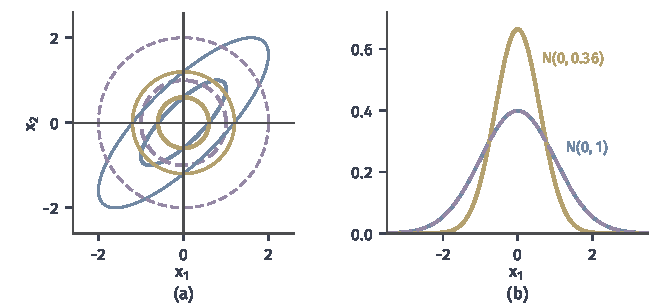
\includegraphics[width=112mm]{figures/07-probability/07-distribution-optimization/matplotlib/dapx-gauss-meanfield/figure.pdf}
 \caption{独立高斯候选逼近相关高斯目标，$\rho=0.8$。(a)等高线$\bm{x}^{\top}\bm{C}^{-1}\bm{x}=c^{2}$，$c=1,2$：目标$\bm{C}=\bm{\Sigma}$（蓝）；按候选加权的最优解$\bm{C}=0.36\,\bm{I}_2$（黄）；按目标加权的最优解$\bm{C}=\bm{I}_2$（紫色虚线）。(b)$X_1$的边缘密度：目标与按目标加权的解都是$\mathcal{N}(0,1)$（蓝线与紫色虚线重合），按候选加权的解是$\mathcal{N}(0,0.36)$（黄）。}
 \label{fig:dapx-gauss-meanfield}
\end{BookInlineFigure}

方差变小会直接影响尾概率。事件$\{\lvert X_1\rvert>1.5\}$在目标与$Q_{\mathrm{r}}$下的概率分别是
\[
 2\bigl(1-\Phi(1.5)\bigr)\approx0.134,\qquad 2\bigl(1-\Phi(1.5/0.6)\bigr)=2\bigl(1-\Phi(2.5)\bigr)\approx0.0124 ,
\]
后者小了十倍以上。所以，即使是族内最优的近似，也可能改变后续任务关心的数值特征；KL的值$0.51$本身不会告诉我们这一点。

把一个方向的最优解放到另一个方向上评价，两者都明显变差。代入上面的公式，
\[
 D_{\mathrm{KL}}(\Pi\Vert Q_{\mathrm{r}})=D_{\mathrm{KL}}(Q_{\mathrm{f}}\Vert\Pi)=\tfrac12\Bigl[\frac{2\rho^{2}}{1-\rho^{2}}+\ln(1-\rho^{2})\Bigr]\approx1.267 .
\]
图~\ref{fig:dapx-rho-curves}画出这些量随$\rho$的变化。$\rho\to\pm1$时，两个变量越来越接近同一个变量，乘积候选能做到的最好程度$-\tfrac12\ln(1-\rho^{2})$趋于无穷，按候选加权所得的方差$1-\rho^{2}$趋于零。

\begin{BookInlineFigure}
 \centering
 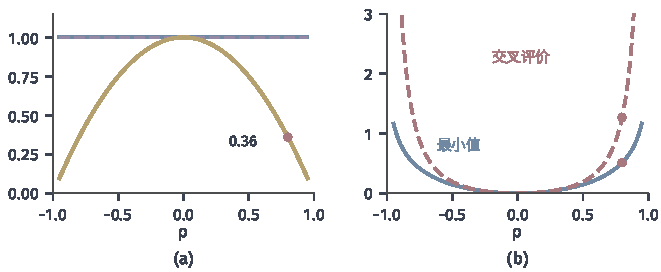
\includegraphics[width=112mm]{figures/07-probability/07-distribution-optimization/matplotlib/dapx-rho-curves/figure.pdf}
 \caption{相关系数的影响。(a)最优独立候选的分量方差：按候选加权为$1-\rho^{2}$（黄），按目标加权为$1$（紫色虚线，与目标边缘方差的蓝线重合）；红点是$\rho=0.8$时的$0.36$。(b)蓝线是两个方向共同的最小值$-\tfrac12\ln(1-\rho^{2})$；红色虚线是交叉评价，即一个方向的最优解在另一个方向上的值。}
 \label{fig:dapx-rho-curves}
\end{BookInlineFigure}

概率表~\eqref{eq:dapx-table}上也有同样的现象，只是形式不同。下一小节将求出，按候选加权的最优乘积是$q_1=q_2=(\tfrac14,\tfrac34)$或$q_1=q_2=(\tfrac34,\tfrac14)$，KL约为$0.4978$，而按目标加权的最优乘积是均匀表。前者让$Q(X_1=X_2)=\tfrac{10}{16}=0.625$，比均匀表的$0.5$更接近目标的$0.9$，代价是把边缘从$\tfrac12$改成了$\tfrac34$。两个方向在同一个乘积限制下各保留了目标的一部分特征，没有一个能全部保留。

\subsection{逐因子的坐标更新}
\label{sec:dapx-cavi}

按候选加权的方向在高斯例子里能直接求解，一般目标则不能。不过乘积结构给了一个好办法：固定其余因子，只调整一个因子，这个子问题有显式的最优解。依次对每个因子这样做，就是\term{坐标上升变分推断}（coordinate ascent variational inference），简称CAVI。“上升”指的是对$\ln Z$的变分下界~\eqref{eq:dapx-lower-bound}上升，等价于对KL下降。

\paragraph{主要思想}
固定$q_k$（$k\neq j$），把它们的乘积记为$q_{-j}$，对应的变量记为$\bm{x}_{-j}$。目标对数密度对$x_j$的依赖，在候选看来是什么样子？最自然的答案是：对其余变量按$q_{-j}$求平均。定义
\begin{equation}
 g_j(x_j)=\mathbb{E}_{q_{-j}}\bigl[\ln\widetilde{\pi}(x_j,\bm{X}_{-j})\bigr] .
 \label{eq:dapx-cavi-g}
\end{equation}
它是在“其余变量服从当前因子”的假定下，$x_j$处目标的平均对数密度。把它取指数并归一化，得到当前因子的更新：
\begin{equation}
 q_j^{\mathrm{new}}(x_j)=\frac{\exp(g_j(x_j))}{\int_{\mathcal{X}_j}\exp(g_j)\,\mathrm{d}\lambda_j} .
 \label{eq:dapx-cavi-update}
\end{equation}
下面的定理说明它恰好是子问题的唯一最优解。先在有限状态、目标处处为正的情形证明，这时所有求和都是有限和，没有可积性问题。

\begin{theorem}[逐因子最优更新]
\label{thm:dapx-cavi}
设每个$\mathcal{X}_k$是有限集，$\widetilde{\pi}(\bm{x})>0$对一切$\bm{x}$成立。固定$q_k$（$k\neq j$），按式~\eqref{eq:dapx-cavi-g}、\eqref{eq:dapx-cavi-update}定义$g_j$与$q_j^{\mathrm{new}}$。则对$\mathcal{X}_j$上任意概率$q_j$，
\begin{equation}
 D_{\mathrm{KL}}(q_j\otimes q_{-j}\Vert\Pi)=D_{\mathrm{KL}}(q_j\Vert q_j^{\mathrm{new}})+c_j ,
 \label{eq:dapx-cavi-identity}
\end{equation}
其中$c_j$只依赖$q_{-j}$与$\widetilde{\pi}$。因此$q_j^{\mathrm{new}}$是固定其余因子时唯一的最优因子。
\end{theorem}

\begin{proof}
记$Q=q_j\otimes q_{-j}$。由式~\eqref{eq:dapx-J-shift}，$D_{\mathrm{KL}}(Q\Vert\Pi)=J(Q)+\ln Z$，只需处理$J(Q)$。乘积分布的对数密度是各因子对数密度之和，所以
\[
 \mathbb{E}_{Q}[\ln q(\bm{X})]=\sum_{x_j}q_j(x_j)\ln q_j(x_j)+\sum_{k\neq j}\sum_{x_k}q_k(x_k)\ln q_k(x_k) .
\]
目标对数密度的期望先对$\bm{x}_{-j}$求和、再对$x_j$求和，由式~\eqref{eq:dapx-cavi-g}，
\[
 \mathbb{E}_{Q}[\ln\widetilde{\pi}(\bm{X})]=\sum_{x_j}q_j(x_j)\sum_{\bm{x}_{-j}}q_{-j}(\bm{x}_{-j})\ln\widetilde{\pi}(x_j,\bm{x}_{-j})=\sum_{x_j}q_j(x_j)g_j(x_j) .
\]

记$Z_j=\sum_{x_j}\exp(g_j(x_j))$，则$g_j(x_j)=\ln q_j^{\mathrm{new}}(x_j)+\ln Z_j$。两式相减，并把与$q_j$无关的项合并：
\[
 J(Q)=\sum_{x_j}q_j(x_j)\ln\frac{q_j(x_j)}{q_j^{\mathrm{new}}(x_j)}-\ln Z_j+\sum_{k\neq j}\sum_{x_k}q_k(x_k)\ln q_k(x_k) .
\]
第一项是$D_{\mathrm{KL}}(q_j\Vert q_j^{\mathrm{new}})$，其余各项不含$q_j$。加上$\ln Z$即得式~\eqref{eq:dapx-cavi-identity}，其中
\[
 c_j=-\ln Z_j+\sum_{k\neq j}\sum_{x_k}q_k(x_k)\ln q_k(x_k)+\ln Z .
\]
由Gibbs不等式，第一项非负，仅在$q_j=q_j^{\mathrm{new}}$时为零。
\end{proof}

更新公式有几处值得注意。第一，用$\widetilde{\pi}$还是$\pi$不影响结果：两者只差常数$\ln Z$，$g_j$随之平移一个常数，取指数归一化后抵消。第二，$\widetilde{\pi}(x_j,\bm{x}_{-j})$是条件密度$\pi(x_j\mid\bm{x}_{-j})$乘以一个不含$x_j$的因子，所以$q_j^{\mathrm{new}}$也正比于$\exp\bigl(\mathbb{E}_{q_{-j}}[\ln\pi(x_j\mid\bm{X}_{-j})]\bigr)$：它是目标条件分布在其余因子下的“对数平均”。这是名称中“平均场”的来源：$x_j$看到的不是其余变量的真实取值，而是它们在当前候选下的平均影响。第三，更新只用到$\ln\widetilde{\pi}$的期望，对目标只需要逐点计算未归一化密度。图~\ref{fig:dapx-factor-update}用概率表~\eqref{eq:dapx-table}演示一次更新。

\begin{BookInlineFigure}
 \centering
 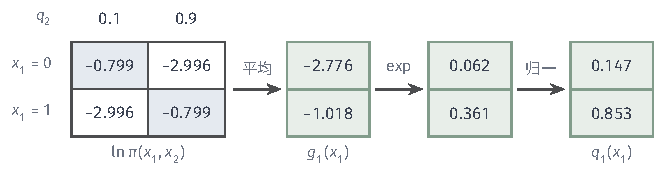
\includegraphics[width=112mm]{figures/07-probability/07-distribution-optimization/tikz/dapx-factor-update/figure.pdf}
 \caption{一次因子更新。左：目标对数概率$\ln\pi(x_1,x_2)$，列上方是当前因子$q_2=(0.1,0.9)$。按$q_2$对每一行加权平均得到$g_1(x_1)$（式~\eqref{eq:dapx-cavi-g}），取指数后归一化，得到新的$q_1=(0.147,0.853)$（式~\eqref{eq:dapx-cavi-update}）。}
 \label{fig:dapx-factor-update}
\end{BookInlineFigure}

\paragraph{高斯目标}
对式~\eqref{eq:dapx-gauss-target}的目标，记精度矩阵$\bm{\Lambda}=\bm{\Sigma}^{-1}$，取未归一化密度
\[
 \ln\widetilde{\pi}(\bm{x})=-\tfrac12\bm{x}^{\top}\bm{\Lambda}\bm{x} .
\]
固定$q_2$，记它的均值为$m_2$。展开二次型，对$X_2$求期望，只保留含$x_1$的项：
\[
 g_1(x_1)=-\tfrac12\Lambda_{1,1}x_1^{2}-\Lambda_{1,2}x_1m_2+\text{常数} .
\]
这是$x_1$的二次函数，取指数后正是高斯密度，配方得到
\[
 q_1^{\mathrm{new}}=\mathcal{N}\Bigl(-\frac{\Lambda_{1,2}}{\Lambda_{1,1}}m_2,\ \frac{1}{\Lambda_{1,1}}\Bigr)=\mathcal{N}\bigl(\rho m_2,\ 1-\rho^{2}\bigr) .
\]
因子是高斯分布这一点不是事先假定的，而是更新公式推出来的；方差$1-\rho^{2}$与上一小节一致，并且不随$q_2$改变。均值的更新是$m_1\leftarrow\rho m_2$，对第二个因子同样有$m_2\leftarrow\rho m_1$。一轮下来$m_2$乘以$\rho^{2}$，从$(m_1,m_2)=(-1.5,2)$出发，第一轮得到$m_1=1.6$，$m_2=1.28$，此后每轮缩小到$0.64$倍，收敛到唯一的最优解$\bm{m}=\bm{0}$。图~\ref{fig:dapx-cavi-gauss}画出这条阶梯形路径。

\begin{BookInlineFigure}
 \centering
 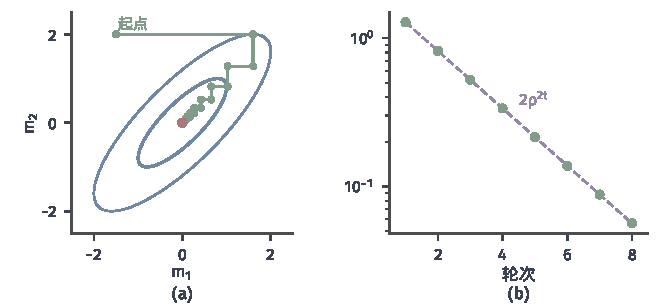
\includegraphics[width=112mm]{figures/07-probability/07-distribution-optimization/matplotlib/dapx-cavi-gauss/figure.pdf}
 \caption{高斯目标上的逐因子更新，$\rho=0.8$。(a)目标等高线（蓝）与因子均值$(m_1,m_2)$的路径（绿）：每步只沿一个坐标方向移动，起点$(-1.5,2)$，红点是最优解$\bm{0}$。(b)每轮结束时的$\lvert m_2\rvert$（绿点，对数纵轴）落在直线$2\rho^{2t}$（紫色虚线）上。}
 \label{fig:dapx-cavi-gauss}
\end{BookInlineFigure}

阶梯的每一步都很短，是因为目标沿对角线拉长：每次只能沿一个坐标轴移动，而沿坐标轴方向目标的“谷”很窄。$\lvert\rho\rvert$越接近$1$，谷越窄，每轮缩小的倍数$\rho^{2}$越接近$1$，收敛越慢。

\paragraph{一般密度}
离开有限状态，定理~\ref{thm:dapx-cavi}的推导需要以下条件，才能让每一步都是有限量的加减：
\begin{itemize}
 \item 对$\lambda_j$几乎处处的$x_j$，$\ln\widetilde{\pi}(x_j,\cdot)$在$q_{-j}$下可积，使$g_j$有定义；
 \item $0<\int\exp(g_j)\,\mathrm{d}\lambda_j<\infty$，使式~\eqref{eq:dapx-cavi-update}能够归一化；
 \item 各因子的$\mathbb{E}_{q_k}\lvert\ln q_k\rvert$有限，$\ln\widetilde{\pi}$在$q_j\otimes q_{-j}$下可积，使Fubini定理允许先对$\bm{x}_{-j}$、再对$x_j$积分。
\end{itemize}
这些条件成立时，证明中的求和换成积分，逐行照搬即可。条件不是形式上的：在高斯目标中，若当前的$q_2$是Cauchy分布，$\mathbb{E}_{q_2}[X_2]$与$\mathbb{E}_{q_2}[X_2^{2}]$都不存在，$g_1$根本没有定义。这时候选的KL也是无穷大，所以实际计算中应当从一个目标值有限的乘积出发，并逐步检查每次更新后上述积分仍然有限。

\paragraph{计算过程}
下面用概率表~\eqref{eq:dapx-table}完整走一遍。两个因子都是$\{0,1\}$上的分布，记$a=q_1(1)$，$b=q_2(1)$。

\needspace{6\baselineskip}
\paragraph{变量}
\begin{itemize}
 \item $\bm{L}\in\mathbb{R}^{2\times2}$：目标对数密度表$L_{x_1,x_2}=\ln\widetilde{\pi}(x_1,x_2)$，只读。
 \item $q_1,q_2$：两个因子，各是长度为$2$的概率向量，在原处更新；二值时只需存$a,b$。
 \item $g$：长度为$2$的工作向量，存放当前正在更新的因子的$g_j$。
 \item $D^{(t)}$：第$t$轮结束时的目标值，用于停止判断；$\varepsilon>0$为容差。
\end{itemize}

\paragraph{初始化}
读入$\bm{L}$，给出第二个因子的初值$q_2^{(0)}$，第一个因子可以任取（它会在第一步被覆盖，只用于计算初始目标值）。例中
\[
 L_{0,0}=L_{1,1}=\ln0.45\approx-0.7985,\qquad L_{0,1}=L_{1,0}=\ln0.05\approx-2.9957 ,
\]
取$q_2^{(0)}=(0.1,\ 0.9)$，$q_1^{(0)}=(0.5,\ 0.5)$，初始目标值$D^{(0)}\approx0.8789$；取$\varepsilon=10^{-4}$。

\needspace{6\baselineskip}
\paragraph{每轮更新}
第$t$轮依次执行：
\begin{enumerate}
 \item \textbf{更新第一个因子。}按式~\eqref{eq:dapx-cavi-g}对每一行用$q_2$加权：
 \[
  g(x_1)=\sum_{x_2}q_2(x_2)L_{x_1,x_2} .
 \]
 再按式~\eqref{eq:dapx-cavi-update}取指数并归一化。数值上先减去$\max g$再取指数，避免下溢。二值时归一化化简为一个logistic函数：
 \[
  a=\frac{1}{1+\exp\bigl(-(g(1)-g(0))\bigr)} .
 \]
 例中第一轮
 \[
  g(0)=0.1\cdot(-0.7985)+0.9\cdot(-2.9957)=-2.7760 ,
 \]
 \[
  g(1)=0.1\cdot(-2.9957)+0.9\cdot(-0.7985)=-1.0182 ,
 \]
 两者之差为$1.7578$，于是
 \[
  a=\frac{1}{1+\mathrm{e}^{-1.7578}}=0.8529,\qquad q_1=(0.1471,\ 0.8529) .
 \]
 这一步后目标值降到$0.5341$。

 \item \textbf{更新第二个因子。}对每一列用新的$q_1$加权：
 \[
  g(x_2)=\sum_{x_1}q_1(x_1)L_{x_1,x_2} ,
 \]
 再取指数并归一化。例中第一轮$2a-1=0.7058$，两个对数概率之差为$\ln0.45-\ln0.05=\ln9=2.1972$，
 \[
  g(1)-g(0)=(2a-1)\ln9=0.7058\cdot2.1972=1.5508 ,
 \]
 于是
 \[
  b=\frac{1}{1+\mathrm{e}^{-1.5508}}=0.8250 .
 \]

 \item \textbf{计算目标值。}乘积分布有四个格，直接求和：
 \[
  D^{(t)}=\sum_{x_1,x_2}q_1(x_1)q_2(x_2)\ln\frac{q_1(x_1)q_2(x_2)}{\pi(x_1,x_2)} .
 \]
 目标只有未归一化形式时改算$J$，停止判断只用差值，不受$\ln Z$影响。例中第一轮$D^{(1)}=0.5117$。

 \item \textbf{停止。}若$D^{(t-1)}-D^{(t)}<\varepsilon$，或已做满预定轮数，输出当前的$q_1,q_2$；否则令$t\leftarrow t+1$，回到第1步。

 例中后续各轮为
 \[
  \begin{array}{cccc}
  t & a & b & D^{(t)}\\
  2 & 0.8067 & 0.7937 & 0.50129\\
  3 & 0.7843 & 0.7772 & 0.49896\\
  4 & 0.7717 & 0.7675 & 0.49824\\
  5 & 0.7641 & 0.7614 & 0.49798\\
  6 & 0.7593 & 0.7576 & 0.49787\\
  7 & 0.7562 & 0.7551 & 0.49783
  \end{array}
 \]
 第$7$轮的下降量$4.3\times10^{-5}$小于$\varepsilon$，停止。
\end{enumerate}

最终得到$q_1\approx(0.244,\ 0.756)$，$q_2\approx(0.245,\ 0.755)$，目标值$0.49783$。继续迭代，$a,b$都趋于$\tfrac34$：二值时更新是$a=\sigma\bigl((2b-1)\ln9\bigr)$，其中$\sigma(z)=1/(1+\mathrm{e}^{-z})$，代入$b=\tfrac34$得$\sigma(\tfrac12\ln9)=\sigma(\ln3)=\tfrac34$，所以$a=b=\tfrac34$是不动点，对应的乘积分布
\[
 Q^{*}=\begin{bmatrix}\tfrac{1}{16}&\tfrac{3}{16}\\\tfrac{3}{16}&\tfrac{9}{16}\end{bmatrix},\qquad D_{\mathrm{KL}}(Q^{*}\Vert\Pi)\approx0.4978 .
\]
停止时的目标值已经与极限相差不到$10^{-4}$，因子却还差约$0.006$：目标值在最优点附近对因子的变化不敏感，用目标值的下降量作停止准则时，因子的精度要另外判断。

\paragraph{收敛与最优性}
由式~\eqref{eq:dapx-cavi-identity}，每次更新一个因子，目标值都不会增加；目标值有下界$0$，所以目标值序列收敛。这是本算法唯一无条件成立的结论。下面三件事要分开看。

第一，目标值收敛不等于因子收敛。在有限状态、各因子始终严格为正的情形，更新映射连续，每个子问题有唯一解，这类分块下降方法的极限点都是驻点；一般情形下需要的条件见\BookChapterRef{chap:block-optimization}{卷五第12章“分块优化”}。

第二，驻点不一定是最小点。从$b^{(0)}=\tfrac12$出发，第一步得到$a=\sigma(0)=\tfrac12$，之后永远停在均匀表，目标值$0.5108$。这是一个鞍点：沿$a=b$方向离开它，目标值下降。

第三，局部最优不一定是全局最优。目标值作为$(a,b)$的函数，对每个坐标单独是凸的（式~\eqref{eq:dapx-cavi-identity}右边是$q_j$的凸函数），但对两个坐标合起来不是凸的。本例有两个最小点$(\tfrac14,\tfrac14)$与$(\tfrac34,\tfrac34)$，从$b^{(0)}=0.2$出发会走到前者。这里两个最小点由对称性给出相同的值；目标不对称时，不同的局部最小点的值一般不同，迭代停在哪里取决于初值。图~\ref{fig:dapx-cavi-table}画出目标值的等高线与两条路径。

\begin{BookInlineFigure}
 \centering
 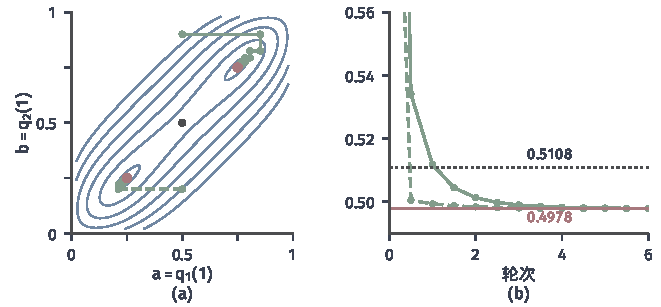
\includegraphics[width=112mm]{figures/07-probability/07-distribution-optimization/matplotlib/dapx-cavi-table/figure.pdf}
 \caption{概率表~\eqref{eq:dapx-table}上的逐因子更新。(a)乘积候选的目标值$D_{\mathrm{KL}}(q_1\otimes q_2\Vert\Pi)$关于$(a,b)$的等高线（蓝），红点是两个最小点$(\tfrac14,\tfrac14)$与$(\tfrac34,\tfrac34)$，深灰点是鞍点$(\tfrac12,\tfrac12)$；绿色实线是从$b^{(0)}=0.9$出发的路径，绿色虚线从$b^{(0)}=0.2$出发，每段折线对应一次因子更新。(b)每次因子更新后的目标值，横轴以轮计；红线是最小值$0.4978$，深灰点线是鞍点的值$0.5108$。}
 \label{fig:dapx-cavi-table}
\end{BookInlineFigure}

计算量取决于$g_j$是否容易求。若$\ln\widetilde{\pi}$是许多只涉及少数变量的项之和，例如前面的成对作用模型，那么$g_j(x_j)$只需要与$x_j$同在一项里的那些变量的因子：对二值变量，它等于$x_j$乘以$h_j+\sum_{k\neq j}J_{j,k}q_k(1)$再加常数（这里约定$J_{j,k}=J_{k,j}$），一次更新的代价与$x_j$参与的项数成正比，一轮的代价与项的总数成正比，而不是$2^{m}$。若$\ln\widetilde{\pi}$把许多变量缠在一个不可分的式子里，$g_j$本身就是一个高维期望，坐标更新也就失去了计算上的好处。
